\documentclass{article}
\usepackage[utf8]{inputenc}
\usepackage{graphicx}
\usepackage{hyperref}
\usepackage{multirow}
\usepackage{amsmath}

\title{Research Methodology UE18CS400SG \\ Unit 4}
\author{Aditeya Baral}
\date{March 2022}

\begin{document}

\maketitle

\section{Interpretation}

Draw inferences from data carefully and write a report, expose relations and processes from findings and communicate analytical findings through a research report.

\subsection{Meaning of Interpretation}

\begin{itemize}
    \item Draw inferences from collects facts after experimental study
    \item Concerned with relationship within data and study beyond data
    \item Establish continuity in research and exploratory concept
    \item Establish explanatory concepts
    \item Appreciate significance of one's findings
    \item Results in hypothesis for experimental research
\end{itemize}

\subsection{Technique of Interpretation}

\begin{enumerate}
    \item Explain how generalization is done and concepts are formulated
    \item Consider extraneous information while interpreting final results
    \item Consult someone with insight into the study, should be honest to point out logical errors in arguments
    \item Interpretation to be done only after considering all relevant factors affecting the problem (to avoid false generalization)
\end{enumerate}

\section{Report Writing}

Case reports, book reviews, essays, editorials, letters, articles etc are report forms apart from scientific reports

\begin{table}[h]
\centering
\begin{tabular}{|l|l|}
\hline
\textbf{Report}                                                                                                                                                                                                                                                                            & \textbf{Research Report}                                                                                                                                                                                                                                                           \\ \hline
\begin{tabular}[c]{@{}l@{}}Collection of facts to give clear and \\ concise information to people who do not have \\ full facts of the subject matter of the report. \\ \\ A report is for a specific audience, types include \\ memos, meeting minutes, expense reports, etc\end{tabular} & \begin{tabular}[c]{@{}l@{}}Written document or oral presentation \\ based on a written document that communicates \\ the purpose, scope, objectives, hypotheses,\\ methodology, findings, limitations and finally \\ recommendations of a research project to others.\end{tabular} \\ \hline
\end{tabular}
\caption{Differences between Report and Research Report}
\label{tab:report-research-report}
\end{table}

\subsection{Categories of Report}

\begin{itemize}
    \item \textbf{Formal} -- meticulously structured, focus on objectivity, organization, deeper details, written in proper style. A \textbf{technical report} is a \textit{formal and organized documentation of the process, progress, results of research created to communicate to an audience important information about the work.}
    \item \textbf{Informal} -- short, free-flowing messages, casual language style
\end{itemize}

\subsection{Steps to Prepare a Report}

\begin{enumerate}
    \item Decide terms of reference
    \item Conduct research
    \item Write outline
    \item Write first draft
    \item Analyze data, record findings
    \item Recommend course of action
    \item Edit and distribute or publish
\end{enumerate}

\subsection{Characteristics of Research Report}

\begin{itemize}
    \item Accuracy, simplicity, conciseness
    \item Comprehensible, readable, complete 
    \item Reliable and economical
    \item Timelines
    \item Logical content
    \item Should also possess:
    \begin{itemize}
        \item Show originality
        \item Ready availability of findings
        \item Appropriate layout in accordance with objective
        \item No grammatical or logical errors
        \item Logical analysis of subject
        \item Index appended at the end
        \item Attractive, neat and clear
    \end{itemize}
\end{itemize}

\subsection{Guidelines for Writing Report}

\begin{enumerate}
    \item Objective
    \item Minimize technical language
    \item Present tense and active voice only
    \item Data confidentiality
    \item Revise and rewrite
    \item Use visual aids
\end{enumerate}

\begin{figure*}[htp]
    \centering
    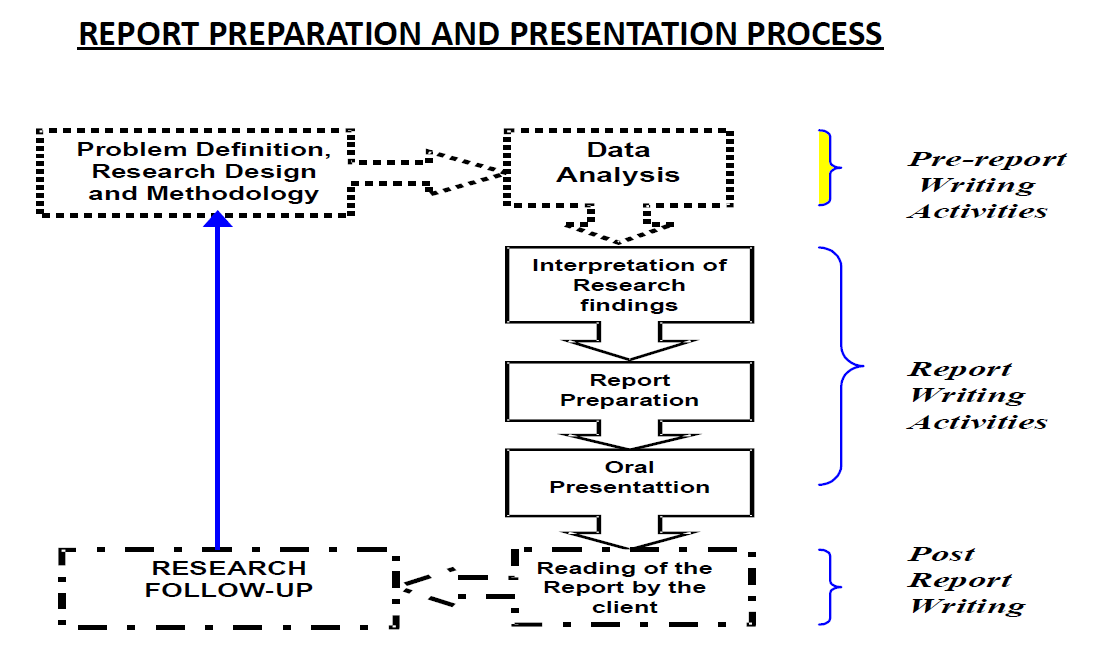
\includegraphics[width=0.7 \linewidth]{img/report-process.png}
    \caption{Report Preparation and Presentation Process}
    \label{fig:report-process}
\end{figure*}

\subsection{Types of Research Reports}

\subsubsection{Technical or Scientific Report}

\begin{itemize}
    \item A document that describes the \textbf{process, progress, or results of a research or the state of a technical or scientific research problem}
    \item Includes summary of results, nature of study, research methodology, details of data, analysis, conclusions, bibliography, appendix, index
\end{itemize}

\subsubsection{Popular Report}

\begin{itemize}
    \item Emphasis on \textbf{simplicity and attractiveness, consists of clear writing, minimal technical and mathematical details, liberal use of charts and diagrams}, large print, cartoons
    \item Includes findings, recommendations, objective, methods, results, appendix
\end{itemize}

\subsubsection{Interim Report}

\begin{itemize}
    \item \textbf{Short report to analyze how project is proceeding before completion}
    \item May contain first results of analysis
    \item Helps sponsoring agency to take action without full report, keeps their interest alive in study and prevent misunderstanding about delays
    \item Important in \textbf{medical trials} to ensure patients are not exposed to danger, and helps researchers find appropriate style of reporting
\end{itemize}

\subsubsection{Summary Report}

\begin{itemize}
    \item Includes a \textbf{brief statement about problem, objective, background information, concise analysis, findings and conclusion}
    \item Aids managers in decision making, important part of business plans
    \item Short, limited size, published in newspapers
\end{itemize}

\subsubsection{Algorithmic Research Report}

\begin{itemize}
    \item Problems exist in reality and solution to these problems can be expressed or obtained as an algorithm
    \item A report that contains the problem, algorithms used to solve the problem and the steps, implementation and findings
\end{itemize}

\subsection{Report Structure}

Abstract, Introduction, Method, Results, Discussion and Conclusion, References are needed. While writing, \textit{start early, remember, read and reflect.}

\begin{enumerate}
    \item \textbf{Preliminary pages} -- title, acknowledgement, abstract, table of contents, list of tables, list of charts and figures
    \item \textbf{Main text} -- introduction, problem statement, literature survey, objectives, limitations, methodology, analysis, conclusion, bibliography, appendix
\end{enumerate}

\subsubsection{Writing Styles}

\begin{itemize}
    \item \textbf{General Report}
    \begin{itemize}
        \item Double-spaced and numbered pages
        \item Each section on new page with bold title
        \item Ends with appendix, includes data, ethics approval form, other information
    \end{itemize}
    \item \textbf{Research Report}
    \begin{itemize}
        \item Title
        \item Letter of transmittal
        \item Table of contents
        \item List of tables, graphs, appendices, exhibits
        \item Executive summary -- findings, conclusions, recommendations
        \item Introduction - background and statement
        \item Approach
        \item Research design -- information need, data collection, scaling techniques, pretesting, sampling, field work
        \item Data analysis - methodology, plan
        \item Results
        \item Limitations
        \item Conclusions and recommendations
        \item Appendix
    \end{itemize}
\end{itemize}

\subsection{Scientific or Research Paper}

\textit{First publication of original research results in a form where peers can repeat experiments and test conclusions in a journal or other document readily available to the scientific community}

\begin{itemize}
    \item \textbf{4 A's} -- \textit{Aim, Awareness, Audience, Articulation}
    \item Author's perspective -- make research known
    \item Reader's perspective -- read about research, findings, assess quality, give feedback, use in their own work
    \item Popular formats (people read in various orders)
    \begin{itemize}
        \item \textbf{IMRaD} -- introduction, methodology, results, discussion
        \item \textbf{IRDaM} -- introduction, results, discussion, methodology
    \end{itemize}
\end{itemize}

Front portion with title, authors and abstract followed by main or core content with IMRaD

\subsubsection{Title}

\begin{itemize}
    \item Few words (keywords), concise, crisp, specific but not narrow
    \item Captures relevant aspects of study without expectations
    \item Captivating, expressive, no extra words (articles, "studies" etc)
    \item Indexed in search engines or databases and important for literature search
\end{itemize}

\subsubsection{Authors}

Greatest to least contribution, head of group is listed last, use same name in all papers

\subsubsection{Abstract}

\begin{itemize}
    \item Summary, widely read and important
    \item Helps identify content of a paper and determine relevance to one's current research work -- should be consistent with main content
    \item Returned by search engines
    \item IMRaD format -- objectives, method, results, conclusion
    \item No figures, charts, tables or references
    \item Do not copy-paste from main content, write after main content is written
\end{itemize}

\subsubsection{Introduction}

\begin{itemize}
    \item Background to understand paper
    \item Highlight relevance and importance of work, no obvious facts
    \item Pose research question and motivate
    \item Short, general to specific content structure
    \item Identify knowledge gap, unknowns, attempts made
    \item How is problem solved, need for solving
    \item Key primary literature, investigate hypothesis
    \item Terms, definitions, clarifications
    \item Strong verbs and active voice, write after main content
\end{itemize}

\subsubsection{Materials and Methodology}

\begin{itemize}
    \item Helps replicate and evaluate work
    \item Describe study design in detail so that work is reproducible
    \item Identify equipment, variables, metrics, analysis, sources, approvals, statistical methods
    \item Reason for methodology (should be sound -- affects credibility and validity of results)
    \item Past tense, active voice, use tables and figures
\end{itemize}

\subsubsection{Results}

\begin{itemize}
    \item Two parts -- description of results and presentation of data
    \item Tables and figures
    \item Present results, do not add too much detail
    \item Organized order -- answer the research questions
    \item No methodology, no raw data (present results/insights)
    \item Short, summarized, past tense
\end{itemize}

\subsubsection{Discussion}

\begin{itemize}
    \item Answer research questions with justification based on results
    \item Explain research gap, questions, summary of findings and how it answers the questions
    \item Discussion and introduction are a pair (answers to questions)
    \item Limitations, relationship with other research, relevance of study
    \item Specific to general, active voice
\end{itemize}

\subsubsection{Tables}

\begin{itemize}
    \item Should be understandable without text, self-explanatory
    \item Uniform format across paper, follow instructions to authors
    \item Add table number and caption
\end{itemize}

\subsubsection{Figures}

\begin{itemize}
    \item Avoid too much information
    \item Ensure font size in image is readable when printed
    \item Add figure number and caption
    \item Follow instructions to authors
\end{itemize}

\subsubsection{Acknowledgement}

Thank people who helped with work but did not make contributions deserving authorship (example, financial support) after taking their prior permission.

\subsubsection{References/Bibliography}

\begin{itemize}
    \item Give credit to other authors and add credibility to your own work
    \item Aids further reading on topic
    \item Use correct reference format
\end{itemize}

\subsubsection{Active and Passive Voice}

Use \textbf{active voice} for emphasis on important parts of a sentence and cut down word count. Use \textbf{passive voice} if the agent is unknown, unimportant or obvious, or is less important than the action or topic.

\subsubsection{Keywords for Research Articles}

\begin{itemize}
    \item Indexed by search engines and used for quick retrieval
    \item Avoid terms in title (use alternate ones), ensure they are relevant
    \item Test keywords before submitting
\end{itemize}

\subsection{Research Impact Factor ($IF$)}

\begin{itemize}
    \item \textbf{Article level metrics} -- views, citations, Altemetric Attention score
    \item \textbf{Journal level metrics} -- impact factor
\end{itemize}

\textit{\textbf{Impact Factor} is the average number of times articles from the journal published in the past two years have been cited in the Journal Citation Report (JCR) year}.

It is calculated by dividing the number of citations in the JCR year by the total number of publications in the last 2 years.

\begin{equation}
    Impact\ Factor (IF)_{year} = \frac{Citations_{year-1} + Citations_{year-2}}{Publications_{year-1} + Publications_{year-2}}
\end{equation}

Impact Factor helps decide where to submit an article for publication, helps libraries make collection development decisions and helps academic departments assess academic productivity and make decisions on promotions and tenure.

\section{Thesis Writing}

\begin{figure*}[htp]
    \centering
    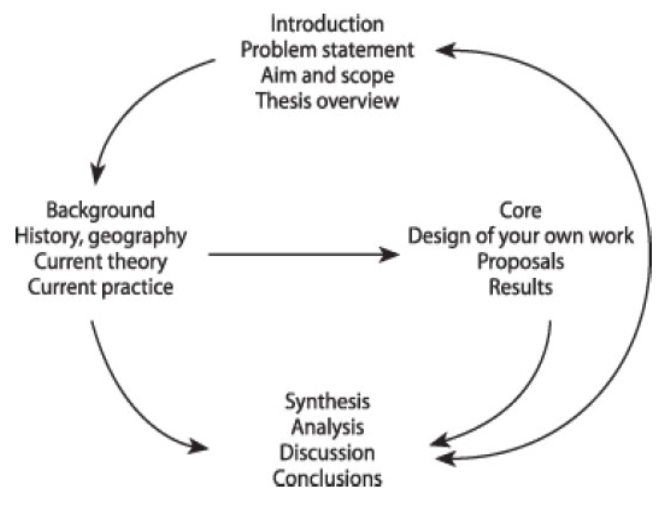
\includegraphics[width=0.7 \linewidth]{img/thesis-structure.png}
    \caption{Thesis Structure}
    \label{fig:report-process}
\end{figure*}

\begin{itemize}
    \item An extended or persuasive argumentation on a research statement, focus, question, issue or topic
    \item Use evidence and reasoning to persuade committee on validity of research
    \item Demonstrate logical, structured, defensible reasoning and original contribution
    \item Submitted as a part of Degree (Bachelor's or Master's)
    \item Consists of main theme, in-depth treatment of aspects and is organized into chapters
    \item Judged by experts
\end{itemize}

\subsection{Parts of a Thesis}

\subsubsection{Title}

\begin{itemize}
    \item Title and subtitle if any
    \item Author names
    \item Whether it is a Bachelor's/Master's thesis
    \item Faculty and department
    \item Place and date of completion
\end{itemize}

\subsubsection{Approval Sheet}

\begin{itemize}
    \item Proves that the authors have passed the requirements needed for the thesis
    \item Signed by thesis/FS advisor, panel and Dean
    \item Also contains grade obtained
\end{itemize}

\subsubsection{Abstract}

\begin{itemize}
    \item Brief summary of contents, not longer than 2 A4 pages
    \item 350 words for Ph.D. and 150 for Masters
    \item Provide important information (and no new information)
\end{itemize}

\subsubsection{Acknowledgement}

Express gratitude to organizations, agencies or individuals who aided researchers in their work.

\subsubsection{Table of Contents}

Topic outline of thesis -- list headings to any level desired. 1" horizontal padding and 2" vertical padding to be used.

\subsubsection{List of Tables/Figures}

Add each list on a separate page -- include number, caption, page number for each item listed.

\subsubsection{Title of Chapters}

1" horizontal padding, 2" from top page, 1" from bottom to footnote, 5" from bottom to page number

\begin{enumerate}
    \item Problem and Background
    \item Review of Related Literature and Studies
    \item Methodology
    \item Presentation, Analysis and Interpretation of Data
    \item Summary, Conclusions and Recommendations
\end{enumerate}

\subsection{Title, Abstract and Keywords}

\textbf{Note} --  This subsection (slides 101 - 108) has mostly repeated content. All slides have been summarised into the following points. Read through.

\begin{itemize}
    \item Words in title and abstract and keywords are indexed in search engines, databases -- used to search for paper
    \item Mostly these sections are freely available online (people read before buying access to paper)
    \item First sections read by reviewers, editors
    \item \textbf{Title} should contain keywords, no filler, repetitive or junk words, crisp and concise, based on answers to research questions
    \item \textbf{Abstract} is marketing tool, helps decide if full paper is required to be read, summary of contents -- why was it done, aim of study, what are the findings
    \begin{itemize}
        \item \textbf{Descriptive} -- used in social sciences and humanities reports, no information about methods and results
        \item \textbf{Informative} -- used in scientific reports, information on background, aim, methods, results and conclusions
        \item \textbf{Structured} -- used in medical sciences and clinical trials, divided into headings (objective, method, results, conclusion)
    \end{itemize}
    \item Write abstract after full paper, include research problem and relevance, how was it solved, main findings, implications of findings. No figures, tables, extra information, abbreviations, citations
    \item Abstract should be consistent with main contents, meets guidelines given to authors, no errors
    \item \textbf{Keywords} should contain repeated or important terms or phrases, and variants of the same as well as abbreviations. Ensure terms are present in an indexing standard in the research discipline and also test on search engines for relevancy.
    
\end{itemize}

\end{document}
